\documentclass[11pt,a4paper,twoside]{book}
%\usepackage[utf8]{inputenc}
%\usepackage[francais]{babel}
%\usepackage[T1]{fontenc}
%\usepackage{amsmath}
%\usepackage{amsfonts}
%\usepackage{amssymb}
%\author{Tigrane Cantat-Moltrecht}
%\title{Atomes de Rydberg piégés}

\usepackage[utf8]{inputenc}
\usepackage{textcomp}
\usepackage[T1]{fontenc}
\usepackage[includeheadfoot, width=144mm,top=23mm,bottom=20mm,bindingoffset=4mm]{geometry}
\renewcommand{\topfraction}{0.5}     % autorise 1/2 page de graphique en haut
\renewcommand{\bottomfraction}{0.3}  % autorise 1/3 page de graphique en bas
\usepackage[fleqn]{amsmath}
\usepackage[french]{babel}
\usepackage{graphicx}
\usepackage[detect-all]{siunitx}
\sisetup{math-micro=\text{µ},text-micro=µ}
\usepackage[font={small}, labelsep=space, labelfont=sf,bf,up,belowskip=14pt,aboveskip=12pt]{caption}
\usepackage{verbatim}
\usepackage[nottoc]{tocbibind}
\usepackage[cmyk]{xcolor} 
\usepackage{tabularx}
\usepackage{fancyhdr}
\usepackage{rotating}

\usepackage{fancyvrb}
\usepackage{adjustbox} 
\usepackage{grffile}
%\include{./0_preamble}
\usepackage{hyperxmp}
\usepackage[pdfpagelayout=TwoPageRight,pdfpagelabels=true]{hyperref}
\hypersetup{
    bookmarks=true,         % show bookmarks bar?
    unicode=true,          % non-Latin characters in Acrobat�s bookmarks
    pdftitle={Laser trapping of circular Rydberg atoms},    % title
    pdfauthor={Tigrane Cantat-Moltrecht},     % author
    pdfsubject={PhD thesis},   % subject of the document
    pdfkeywords={Rydberg} {Atom chip} {Quantum simulation}, % list of keywords
    pdfnewwindow=false,      % links in new window
    colorlinks=true,       % false: boxed links; true: colored links
    linkcolor=black,          % color of internal links
    citecolor=green,        % color of links to bibliography
    filecolor=magenta,      % color of file links
    urlcolor=cyan           % color of external links
}
\usepackage{booktabs}
\usepackage{csquotes}
\csname endofdump\endcsname
\usepackage{enumitem}
\usepackage{setspace}
\newcommand\epigraph[3]{
	\vspace{-2em}\hfill{}\begin{minipage}{#1}{\begin{spacing}{0.9}
				\small\noindent\textit{#2}\end{spacing}
			\vspace{1em}
			\hfill{}{--- #3}}\vspace{6em}
			\end{minipage}\\
			
			\noindent}
\usepackage{afterpage}
\usepackage{braket}
%\usepackage{physics}

\usepackage[backend=biber,style=phys,%
articletitle=true,biblabel=brackets,chaptertitle=true,pageranges=false
]{biblatex}
\DeclareFieldFormat{titlecase}{{#1}}
\usepackage{chngcntr}
\addbibresource{tcm_these.bib}
%\usepackage{fontspec}
\linespread{1.05}
%\usepackage{unicode-math}
%\setmainfont
%[ BoldFont     = TeX Gyre Pagella-Bold,
%ItalicFont     = TeX Gyre Pagella-Italic ,
%BoldItalicFont = TeX Gyre Pagella-Bold Italic ]
%{TeX Gyre Pagella-Regular}
%\setmathfont{TeX Gyre Pagella Math}
%\setmathfont[range=\mathcal]{TeX Gyre Termes  Math}
%\setmathfont[range=\sqrt]{Asana Math}
%\setmathfont[range=\tilde]{Asana Math}
\newcommand{\CoverName}{Cover}%
\newcommand{\BackCoverName}{Back Cover}%
\title{Atomes de Rydberg piégés}
\usepackage{coverpages}
\logos{}{}{}%./logo/logo.pdf}{}{} 
\author{Tigrane Cantat-Moltrecht}
\thesis{THÈSE DE DOCTORAT \protect\\DE L'ÉCOLE NORMALE SUPÉRIEURE}
\specialite{PHYSIQUE QUANTIQUE}
\ecoledoct{\og Physique en Île-de-France\fg}
\lab{DÉPARTEMENT DE PHYSIQUE DE L'ÉCOLE NORMALE SUPÉRIEURE \\ LABORATOIRE KASTLER BROSSEL}
\title{{Atomes de Rydberg circulaires piégés}}
\phdname{DOCTEUR DE L'ÉCOLE NORMALE SUPÉRIEURE}
\date{décembre 2017}
\jury{
Dr. & Michel BRUNE & Directeur de thèse \\	
Dr. & ?? & Rapporteur \\
Pr. & ?? & Rapporteur \\
Dr. & ??  & Examinateur    \\
Pr. & ?? & Examinateur \\
Pr. & ?? & Examinateur
}
\titlefr{titre en français}
\resume{résumé en français}
\motscles{mots clé en français}


\titleen{English title}
\abstract{English abstract}
\keywords{English keywords}

%%%%%%%%%%%%%%%%%%%%%%%%%------------
\begin{document}
\newcommand{\numv}[1]{\num[output-decimal-marker={,}]{#1}~}
\newcommand{\SIv}[2]{\SI[output-decimal-marker={,}]{#1}{#2}~}
\newcommand{\SIvv}[2]{\SI[output-decimal-marker={,}]{#1}{#2}}
\newcommand{\Kel}{\si{\kelvin}}
\newcommand{\mK}{\si{\milli\kelvin}}
\newcommand{\uK}{\si{\micro\kelvin}}
\newcommand{\citefr}[1]{\cite{#1}}
\renewcommand{\vec}[1]{\mathbf{#1}}
\newcommand{\dip}{d}
\newcommand{\VdW}{van der Waals }
\newcommand{\umx}{\si{\um^6} }
\newcommand{\Rb}[1]{${}^{#1}$Rb}
\newcommand{\Ryd}{\textnormal{Ryd }}
\newcommand{\pdt}{\partial_t}
\newcommand{\eff}{\textnormal{eff }}
\newcommand{\Id}{\mathbb{I}}
\renewcommand{\thefootnote}{\fnsymbol{footnote}}
\renewcommand \thechapter{\Roman{chapter}}
\newcommand{\kb}{\mathrm{k_B}}


\frontmatter
\pagenumbering{roman}
\thispagestyle{empty}
%\topskip0pt
\vspace*{0.2\textheight}
\begin{center}
\emph{To ???}
\end{center}
\vspace*{\fill}\clearpage
\makeatletter
\let\ps@plain\ps@empty

\makeatother

\include{}%0_Acknowledgement}
\tableofcontents
\thispagestyle{fancyplain}
\listoffigures
\listoftables
\thispagestyle{fancyplain}
%%\pagebreak
\mainmatter
\pagenumbering{arabic}

\chapter*{Introduction}\label{chapter:intro}
\addcontentsline{toc}{chapter}{Introduction}
\markboth{Introduction}{Introduction}
\include{}%0_intro}

%\chapter{Atomes de Rydberg : à bas $l$ ou circulaires}
%\label{part:Rydberg}




%\chapter{Atomes de Rydberg alcalins en interaction}
%\label{chapter:Rydberg}

\chapter{Atomes de Rydberg alcalins en interaction}
\label{chapter:Rydberg}
%Atomes de Rydberg : à bas $l$ ou circulaires

\section{Théorie générale des Rydberg}
	\subsection*{Hamiltonien de l'atome d'hydrogène}
		\noindent particularités aux grands $n$
	\subsection*{Défaut quantique : comment passer aux alcalins}
		\noindent le défaut quantique comme un $n$ effectif
		\noindent quantitativement : $\delta_{n,l,j}$ pour les niveaux qui nous concernent
	\subsection*{Niveaux à bas $l$}
		\noindent description rapide des spécificités et schéma de niveaux
		\noindent taille, dipole
		\noindent transitions vers niveaux proches, émission spontanée, temps de vie
	\subsection*{Niveaux circulaires}
		\noindent description rapide des spécificités et schéma de niveaux
		\noindent taille, dipole
		\noindent transitions vers niveaux proches, émission spontanée, temps de vie
	\subsection*{Les grandes caractéristiques des Rydberg}
		\noindent gigantisme du dipole, sensibilité au champ EM, interactions
		\noindent lois d'échelle

\section{Atomes de Rydberg en interaction}
	\subsection*{Deux atomes de Rydberg}
		\noindent hamiltonien d'interaction
		\noindent dipole-dipole
		\noindent Van der Waals
		\noindent interaction d'échange
	\subsection*{les interactions entre Rydberg de bas $l$}
		\noindent origine du $C_6$ pour 60s-60s et $C_6/A_6$ avec les voisins
		\noindent blocage dipolaire et facilitation
	\subsection*{les interactions entre Rydberg circulaires}
		\noindent $C_6$ pour 50c-50c et $C_6/A_6$ avec les voisins
\section{Atomes de Rydberg en interaction}
Dans cette thèse, nous allons nous intéresser aux interactions entre plusieurs atomes de Rydberg voisins, dans des niveaux identiques ou proches en énergie.
Le reste de ce chapitre est consacré au calcul de ces interactions et à leur application aux deux cas qui nous concernent : autour des niveaux 60S et 50C.

	\subsection{Deux atomes de Rydberg qui se parlent}
L'opérateur de moment dipolaire entre deux niveaux de Rydberg proches est grand, comme nous l'avons évoqué.
En cela, les atomes de Rydberg sont de très bonnes antennes pour le rayonnement électromagnétique lorsque celui-ci est résonant avec les fréquences de transition entre niveaux proches.
Cette caractéristique s'accentue fortement lorsque le nombre quantique principal augmente, car le moment dipolaire varie en $n^{*2}$.
Ces grands moments de transition dipolaires font aussi apparaître une interaction importante entre deux atomes de Rydberg différents : bien qu'ils restent des objets neutres électriquement, ces grands dipôles se voient très bien de loin.
En électromagnétisme classique, le terme de couplage entre deux dipôles électriques s'écrit \cite{TXT_JACKSON}
\begin{equation}\label{eq:classicDipole}
V_{dd}(\vec{r}) = \frac{1}{4\pi\epsilon_0 r^3} \left( \vec{d_1}\cdot \vec{d_2} - 3(\vec{d_1}\cdot \frac{\vec{r}}{r})(\vec{d_2}\cdot\frac{\vec{r}}{r}) \right)
\end{equation}
où $\vec{d_1}$ décrit le premier dipôle, $\vec{d_2}$ le deuxième dipôle et $\vec{r}$ le vecteur d'espace qui les sépare.
On peut alors écrire, par analogie, le hamiltonien d'interaction entre deux atomes en remplaçant les dipôles classiques par les opérateurs dipôle électrique de chaque atome.
La distance entre les atomes sera cependant traitée de façon classique, en supposant que la distance entre les atomes est très grande devant l'extension spatiale de leurs fonctions d'onde. C'est ce qu'on appelle l'approximation dipolaire.
Le potentiel d'interaction dipolaire s'écrit dans ce cas
\begin{equation}\label{eq:quantDipole}
\begin{aligned}
\hat{V}_{dd}(\vec{r}) &= \frac{1}{4\pi\epsilon_0 r^3} \left( \vec{\hat{d}_1}\cdot \vec{\hat{d}_2} - 3(\vec{\hat{d}_1}\cdot \frac{\vec{r}}{r})(\vec{\hat{d}_2}\cdot\frac{\vec{r}}{r}) \right) \\
&= \frac{q^2}{4\pi\epsilon_0 r^3} \left( \vec{\hat{r}_1}\cdot \vec{\hat{r}_2} - 3(\vec{\hat{r}_1}\cdot \frac{\vec{r}}{r})(\vec{\hat{r}_2}\cdot\frac{\vec{r}}{r}) \right).
\end{aligned}
\end{equation}
%
Remarquons que ce terme dépend du produit des opérateurs de transition dipolaire électrique de chaque atome. L'interaction entre atomes de Rydberg varie donc comme $(n^{*2})^2 = n^{*4}$.

\bigskip
Calculer l'interaction entre deux atomes de Rydberg revient à diagonaliser le hamiltonien total du système des deux atomes dans l'espace de Hilbert des états possibles pour la paire d'atomes.
Sans autre \textit{a priori}, une base naturelle pour cet espace est le produit tensoriel $\ket{R_1}\otimes\ket{R_2}$ des états de chaque atome.
Dans cette base, le hamiltonien du système s'écrit
\begin{equation}\label{eq:hamilt2atoms}
\hat{H} = \hat{H}_{0,1} + \hat{H}_{0,2} + \hat{V}_{dd}(\vec{r})
\end{equation}
où $\hat{H}_{0,i}$ est le hamiltonien de l'atome $i$ isolé.

En l'absence de champ électrique ou magnétique extérieur, l'axe de quantification pour les niveaux de chaque atome n'est pas déterminé.
Il semble naturel de choisir alors comme axe de quantification le vecteur qui sépare les atomes.
Dans cette géométrie, le potentiel d'interaction dipolaire prend la forme
\begin{equation}\label{eq:Vdd_rr1r2}
\begin{aligned}
\hat{V}_{dd}(\vec{r})=&
-\frac{q^2}{4\pi\epsilon_0}\frac{\hat{r}_1\hat{r}_2}{r^3}\frac{4\pi}{3} \times
\left( \hat{Y}^1_1(\theta_1,\phi_1) \hat{Y}^{-1}_1(\theta_2,\phi_2) \right. \\
&\left. + \hat{Y}^{-1}_1(\theta_1,\phi_1) \hat{Y}^{1}_1(\theta_2,\phi_2)
+ 2\hat{Y}^{0}_1(\theta_1,\phi_1) \hat{Y}^{0}_1(\theta_2,\phi_2)
\right)
\end{aligned}
\end{equation}
où les $Y^{m_l}_l$ sont les harmoniques sphériques, solutions des équations de Legendre \cite{TXT_COHEN1FR}.
Dans cette base, l'opérateur $\hat{V}_{dd}$ préserve le nombre quantique magnétique total $M=m_{j1}+m_{j2}$.
Cette condition définit un sous-espace des niveaux de même $M$ pour la paire d'atomes, sous-espace qui a une dimension infinie.
Il sera donc nécessaire, pour calculer l'interaction entre les deux atomes, de tronquer ce sous-espace.
Dans le sous-espace tronqué, nous pouvons diagonaliser le hamiltonien \eqref{eq:hamilt2atoms} pour chaque distance interatomique $r$.

\subsection{Deux atomes dans le même niveau de Rydberg}
Dans le cas de deux atomes dans le même niveau de Rydberg $a$, la règle de sélection $\Delta l = \pm 1$ impose que $\braket{aa|\hat{V}_{dd}|aa} = 0$.
L'opérateur d'interaction dipolaire n'agit donc sur la paire $\ket{aa}$ que comme une perturbation de second ordre, \textit{via} le couplage à des niveaux de paire intermédiaires $\ket{cd}$.
La figure \eqref{fig:Dip_aacd} représente ce couplage au second ordre.
L'énergie d'interaction résultant de cette perturbation prend la forme
\begin{equation}\label{eq:VdW_aacd}
C_{aa}(r)=\sum_{\ket{cd}}{\frac{\braket{aa|\hat{V}_{dd}|cd}\braket{cd|\hat{V}_{dd}|aa}}{2E_a - E_c - E_d}}  = \frac{C_{6,aa}}{r^6}
\end{equation}
où $E_i$ est l'énergie d'un atome de Rydberg individuel dans l'état $i$.
L'interaction dipolaire prend donc la forme d'une interaction de Van der Waals en $1/r^6$, avec un coefficient valant $C_{6,aa}$.

\begin{figure}[!h]
\centering

\includegraphics[width=0.3\linewidth]{figures/dipole_coupling_aacd}
\caption[Couplage dipolaire entre mêmes niveaux de Rydberg]{Schéma du couplage dipolaire entre deux atomes dans des niveaux de Rydberg $a$ identiques : le couplage s'effectue au second ordre \textit{via} les niveaux $c$ et $d$.}
\label{fig:Dip_aacd}
\end{figure}

La situation se complique lorsque l'un des niveaux intermédiaires $\ket{cd}$ est quasi-dégénéré avec le niveau $\ket{aa}$, c'est-à-dire lorsque $\braket{aa|\hat{V}_{dd}|cd} \gg |2E_a-E_c-E_d|$.
Le développement perturbatif est en effet invalidé sous cette condition et il est nécessaire de traiter le problème différemment.
Si $\ket{c}=\ket{d}$, alors le sous-espace à observer est composé des deux états $\ket{aa}$ et $\ket{cc}$ et l'on a $E_c\simeq E_a$.
Le hamiltonien d'interaction s'écrit alors
\begin{equation}\label{eq:forster_aacc}
H_{aa-cc} = \bordermatrix{~ 	&\ket{aa} 	& \ket{cc} \cr
	\ket{aa}		&2E_a 		& \frac{\Braket{aa|V_{dd}|cc}}{r^3}	\cr 
	\ket{cc} 		& \frac{\Braket{aa|V_{dd}|cc}}{r^3} 		&2E_a\cr} \ .
\end{equation}
%
Les états propres de ce hamiltonien sont les combinaisons symétrique et antisymétrique $(\ket{aa}\pm\ket{cd})/\sqrt{2}$, et présentent les énergies propres
\begin{equation}\label{eq:forster_aacc_energies}
2E_a \pm \Delta E_{dd} = 2E_a \pm\frac{\braket{aa|V_{dd}|cc}}{r^3}= 2E_a \pm\frac{C_{3,aa}}{r^3}.
\end{equation}

Si, au contraire, $\ket{c}\neq \ket{d}$, on est alors en présence de trois états dégénérés : $\ket{aa}$, $\ket{cd}$ et $\ket{dc}$.
Il est utile de réécrire ceux-ci en combinant $\ket{cd}$ et $\ket{dc}$ symétriquement et anti-symétriquement en $\ket{C}=(\ket{cd}+\ket{dc})/\sqrt{2}$ et $\ket{NC}=(\ket{cd}-\ket{dc})/\sqrt{2}$.
En effet, $\hat{V}_{dd}$ ne couple pas le niveau $\ket{aa}$ avec le niveau $\ket{NC}$.
On peut donc appliquer le traitement réservé jusqu'ici au cas $\ket{c}=\ket{d}$ en remplaçant $\ket{cc}$ par $\ket{C}$.
Nous obtenons donc deux états propres $(\ket{aa}\mp \ket{C})/\sqrt{2}$ avec les énergies
\begin{equation}\label{eq:forster_aacd_energies}
2E_a \pm \Delta E_{dd} = 2E_a \pm\frac{\braket{aa|V_{dd}|C}}{r^3}= 2E_a \pm\frac{\braket{aa|V_{dd}|cd}}{r^3}= 2E_a \pm\frac{C_{3,aa}}{r^3}.
\end{equation}
Ces cas particuliers sont analogues à ce que l'on appelle dans d'autres contextes les résonances de Förster \cite{MX_BROWAEYSDD14}.

\subsection{Deux atomes dans des niveaux de Rydberg différents}
\label{subsec:interaction_diff_levels}
Intéressons-nous désormais aux interactions entre deux atomes de Rydberg dans les états $a$ et $b$.
Il y a alors deux états de paire dégénérés $\ket{ab}$ et $\ket{ba}$.
De même que précédemment, les termes de couplage $\braket{ab|\hat{V}|ab}=\braket{ba|\hat{V}|ba}$ sont nuls.
L'on peut tout de même introduire un opérateur potentiel effectif $V_{eff}$ pour le système à deux niveaux $\ket{ab}$ et $\ket{ba}$, qui tiendra compte des couplages de second ordre avec des états intermédiaires.
Les éléments de matrice de $V_{eff}$ sont
%
\begin{equation}\label{eq:Cab_Aab}
\begin{aligned}
&C_{ab}=\braket{ab|V_{eff}|ab}=\braket{ba|V_{eff}|ba} \\
\text{et} &\\
&A_{ab}=\braket{ab|V_{eff}|ba}=\braket{ab|V_{eff}|ba}.
\end{aligned}
\end{equation}
%
L'hamiltonien d'interaction s'écrit sous forme matricielle
\begin{equation}\label{eq:MatrixCab_Aab}
V_{eff} = \bordermatrix{~ 	&\ket{ab} 	& \ket{ba} \cr
	\ket{ab}		&C_{ab} 		&A_{ab}	\cr 
	\ket{ba} 		&A_{ab} 		&C_{ab} \cr} \ .
\end{equation}
%
Les termes diagonaux de ce hamiltonien représentent l'interaction directe d'un état de paire avec lui-même, qui se calcule donc comme une perturbation de second ordre \textit{via} les niveaux intermédiaires $\ket{cd}$.
Comme c'était le cas pour deux atomes dans le même état de Rydberg, cette interaction prend la forme de Van der Waals avec un coefficient $C_{6,ab}$ :
\begin{equation}\label{eq:VdW_abab}
C_{ab}(r)=\sum_{\ket{cd}}{\frac{\braket{ab|\hat{V}_{dd}|cd}\braket{cd|\hat{V}_{dd}|ab}}{E_a + E_b - E_c - E_d}}  = \frac{C_{6,ab}}{r^6}.
\end{equation}

Les termes non-diagonaux $A_{ab}$ correspondent eux à une interaction au cours de laquelle les deux atomes échangent leurs états.
Si la transition $a\rightarrow b$ est autorisée par les règles de sélection dipolaires, alors cette interaction d'échange est un couplage \textit{direct} de $\ket{ab}$ et $\ket{ba}$.
Il varie donc comme un potentiel dipolaire en $1/r^3$.
Dans le cas contraire, l'interaction d'échange sera un couplage dipolaire indirect au second ordre, variant donc en $1/r^6$, voire d'ordre supérieur, comme l'illustre la figure \eqref{fig:Dip_abab}.

\begin{figure}[!h]
\centering
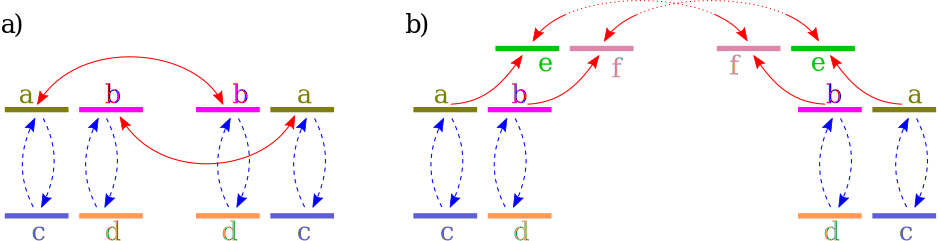
\includegraphics[width=0.9\linewidth]{figures/dipole_coupling_abab}
\caption[Couplage dipolaire entre niveaux de Rydberg différents]{Schéma du couplage dipolaire entre deux atomes dans des niveaux de Rydberg différents $a$ et $b$ : le couplage $ab-ab$ s'effectue au second ordre \textit{via} les niveaux $c$ et $d$. Le couplage $ab-ba$ peut s'effectuer à l'ordre 1(\textbf{a}), à l'ordre 2 via des niveaux intermédiaires $e$ et $f$(\textbf{b}), ou plus encore.}
\label{fig:Dip_abab}
\end{figure}


Lorsque les termes d'échange $A_{ab}$ deviennent comparables aux termes d'interaction directe $C_{ab}$, il peut être judicieux de diagonaliser le hamiltonien effectif \eqref{eq:MatrixCab_Aab}.
En effet, les états propres de celui-ci, qui sont les combinaisons symétrique et anti-symérique $(\ket{ab}\pm \ket{ba})/\sqrt{2}$, ne sont plus dégénérés et présentent respectivement des déplacements d'énergie
\begin{equation}
\label{eq:shift_abab}
\Delta E_{dd} = C_{ab} \mp A_{ab}.
\end{equation}

Afin d'illustrer les calculs d'interaction que nous venons de présenter, nous allons les appliquer à nos deux exemples que sont le niveau 60S et le niveau 50C.
Dans les deux cas, le calcul numérique consiste à diagonaliser le hamiltonien \eqref{eq:hamilt2atoms} à tous les ordres perturbatifs, en limitant l'espace de Hilbert à quelques centaines d'états de paire et sous l'approximation dipolaire.

\subsection{Les interactions dipolaires du niveau 60S}

\subsubsection*{L'interaction 60S-60S}
Dans le cas de l'état $\ket{60\text{S},60\text{S}}$, le terme dominant dans la somme \eqref{eq:VdW_aacd} permettant de calculer le coefficient de Van der Waals $C_{6,\text{60S60S}}$ est le coulage avec les paires $\ket{60\text{P}_j,59\text{P}_j}$.
Puisque $E_{60S}-E_{59P}>E_{60P}-E_{60S}$, le dénominateur du terme de couplage principal dans \eqref{eq:VdW_aacd} est positif.
On en déduit que l'interaction 60S-60S, et plus généralement toute interaction dipolaire nS-nS, est toujours répulsive.
%
\begin{figure}[!h]
\centering
\includegraphics[width=0.8\linewidth]{figures/VdW_60S60S}
\caption[Interaction dipolaire 60S-60S]{Déplacement en énergie de la paire 60S-60S par interaction de Van der Waals. Les différents sous-niveaux $\ket{60\text{P}_j,59\text{P}_j}$ sont représentés. L'échelle de couleur représente le carré de la projection sur l'état non perturbé $\ket{60\text{S},60\text{S}}$.
L'insert représente le déplacement d'énergie en échelle log-log et son ajustement sous la forme de Van der Waals.}
\label{fig:VdW_60s60s}
\end{figure}
%
Le calcul numérique de l'interaction 60S-60S et son ajustement sous la forme de Van der Waals, représentés en figure \eqref{fig:VdW_60s60s}, donnent la valeur
\begin{equation}
\label{eq:C660S}
C_{6,60S60S} = \numv{137.6(1)}\si{\giga\hertz\raiseto{6}\micro\meter}.
\end{equation}

L'ajustement de Van der Waals fonctionne très bien aux distances supérieures à $\sim\SIvv{3}{ \micro\meter}$.
Cependant, aux très courtes distances, la paire $\ket{60\text{S},60\text{S}}$ est très fortement couplée aux niveaux $\ket{60\text{P}_j,59\text{P}_j}$.
La distance critique est celle à laquelle le couplage dipolaire est aussi fort que la différence d'énergie entre les deux états de paire non perturbés, soit ici $\sim \SIv{2}{\giga\hertz}$.
En deçà de cette distance, les états propres du hamiltonien s'éloignent de plus en plus de l'état non perturbé $\ket{60\text{S},60\text{S}}$ et l'interaction évolue vers une interaction dipolaire résonante en $1/r^3$.

\subsubsection*{Les interactions 60S-$nl$}
Le niveau 60S interagit également avec des états de $n$ et $l$ différents.
Il convient alors, comme nous l'avons montré en \eqref{subsec:interaction_diff_levels}, de calculer non seulement les coefficients de Van der Waals $C_{ab}$, mais aussi les éléments de matrice d'échange $A_{ab}$.
De plus, il est possible ici d'avoir des termes d'échange dûs à un couplage dipolaire direct et qui varient donc en $r^3$.

\begin{figure}[h]
\centering
\includegraphics[width=0.8\linewidth]{figures/VdW_60S60P}
\caption[Interaction dipolaire 60S-60P$_{3/2}$]{Énergie de la paire 60S-60P$_{3/2}$ en présence de l'interaction dipolaire.
Les branches inférieure et supérieure correspondent respectivement aux superpositions symétrique et antisymétrique des deux niveaux de départ.
L'échelle de couleur représente le carré de la projection sur l'état non perturbé $\ket{60\text{S},60\text{P}_{3/2}}$.
La ligne pointillée représente le déplacement en énergie dû à l'interaction directe.
L'insert représente le déplacement d'énergie ainsi que le terme d'échange en échelle log-log et leurs ajustements en $1/r^6$ et $1/r^3$ respectivement.
}
\label{fig:VdW_60S60P}
\end{figure}

La figure \eqref{fig:VdW_60S60P} montre par exemple le résultat du calcul de l'interaction dipolaire pour une paire 60S-60P$_{3/2}$.
Aux grandes distances, l'état de la paire est projeté uniformément sur les deux superpositions symétrique et anti-symétrique.
Aux plus courtes distances cependant, d'autres niveaux contaminent la paire, qui n'est plus dans une superposition de $\ket{60\text{S}}$ et $\ket{60\text{P}_{3/2}}$.

En procédant dela même façon, on peut obtenir les coefficients d'interaction dipolaire pour n'importe quelle paire 60S-$nl$. La table \eqref{tab:VdWcoef_60S_nl} synthétise les résultats des calculs numériques pour plusieurs paires contenant le niveau 60S.

\begin{table}[h!]
	\centering
	\caption[Coefficients de Van der Waals 60S-nl]{Coefficients de Van der Waals pour les interactions de paire entre le niveau 60S et différents niveaux voisins $nl$.}
	\label{tab:VdWcoef_60S_nl}
	\begin{tabular}{c c c c}
		\toprule\midrule
%		\multicolumn{1}{c}{  }
%		&\multicolumn{1}{c}{\text{temps de vie à }\numv{0}\si{\kelvin}}
%		&\multicolumn{1}{c}{\text{temps de vie à }\numv{4.2}\si{\kelvin}}
%		&\multicolumn{1}{c}{\text{temps de vie à }\numv{300}\si{\kelvin}}
%		\\ 
		{ }&$C_6$ (\si{\giga\hertz\raiseto{6}\micro\meter}) & $A_6$ (\si{\giga\hertz\raiseto{6}\micro\meter}) & $A_3$ (\si{\giga\hertz\raiseto{3}\micro\meter})
		\\
		\midrule
		$60\text{S}_{1/2}, 60\text{S}_{1/2}$
		&$\SIv{137.6}{}$
		&$\SIv{0}{}$
		&$\SIv{0}{}$\\
		$60\text{S}_{1/2}, 57\text{S}_{1/2}$
		&$\SIv{-43.265}{}$
		&$\SIv{0.325}{}$
		&$\SIv{0}{}$\\
		$60\text{S}_{1/2}, 61\text{S}_{1/2}$
		&$\SIv{290.125}{}$
		&$\SIv{246.475}{}$
		&$\SIv{0}{}$\\
		$60\text{S}_{1/2}, 60\text{P}_{3/2}$
		&$\SIv{7.976}{}$
		&$\SIv{0}{}$
		&$\SIv{4.411}{}$\\
		\midrule
		\bottomrule
 	\end{tabular}
\end{table}



\subsection{Les interactions dipolaires du niveau 50C}
	
\noindent L'interaction dipolaire entre atomes de Rydberg de très grand moment cinétique est rendue plus complexe du fait de leur forte anisotropie.
En effet, l'interaction entre deux dipôles dépend de l'orientation relative de ceux-ci.
Dans le cas des niveaux $l=0$ tel que le 60S, le problème ne se posait pas car ces niveaux sont à symétrie sphérique.
Dès lors que l'on s'intéresse à l'interaction entre des niveaux à symétrie cylindrique, il est indispensable de savoir comment les atomes s'orientent l'un par rapport à l'autre.
L'interaction dipolaire entre atomes circulaires est encore compliquée par l'introduction d'un champ électrique extérieur, qui déplace et déforme les niveaux par effet Stark.
Le détail de l'interaction dipolaire entre atomes circulaires en présence d'un champ sera discuté au chapitre \ref{chapter:circsim}, mais nous prendrons le temps ici de développer la situation la plus simple :
celle de deux atomes dans le niveau 50C dont les deux orbites sont contenues dans le même plan, comme l'illustre la figure \eqref{fig:double_torus}.
%
\begin{figure}[!h]
\centering
\vspace{1em}
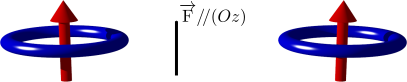
\includegraphics[width=.8\linewidth]{figures/double_torus.png}
\caption[Deux atomes circulaires côte à côte]{Représentation de deux atomes de Rydberg circulaires dont les orbites sont dans le même plan.
Les tores bleus représentent les orbites électroniques et les flèches rouges la direction du moment cinétique.
Si l'on imagine que le dessin est à l'échelle, alors les atomes sont ici séparés d'une distance d'environ \SIv{660}{\nm}.}
\label{fig:double_torus}
\end{figure}
%
Comme il a été dit en \ref{sec:circ_parabol}, les atomes de Rydberg circulaires ont besoin d'un champ électrique extérieur pour se stabiliser.
Nous imposerons donc un champ de \SIvvSym{1}{\V\per\cm}, qui définit l'axe de quantification, parallèle aux flèches rouges sur la figure \eqref{fig:double_torus}.

Les règles de sélection étant toujours valides, le couplage se fait \textit{a priori} à l'ordre deux, et l'équation \eqref{eq:VdW_aacd} permet d'en extraire le coefficient de Van der Waals comme nous l'avons fait pour l'interaction 60S-60S.
Cependant, l'équation \eqref{eq:Vdd_rr1r2} ne prend plus la même forme dans la base parabolique et le moment magnétique total $M$ de la paire atomique n'est plus conservé, ce que doit prendre en compte le calcul numérique.

\begin{figure}[!h]
\centering
\includegraphics[width=1\linewidth]{figures/VdW_50C50C_1Vcm}
\caption[Interaction dipolaire 50C-50C]{Déplacement en énergie de la paire 50C-50C placés côte à côte (cf fig\eqref{fig:double_torus}) par interaction dipolaire, sous un champ électrique de $\SIvv{1}{\V / \cm}$. L'échelle de couleur représente le carré de la projection sur l'état non perturbé $\ket{50\text{C} 50\text{C}}$ de l'état propre du hamiltonien qui le suit adiabatiquement.
Le comportement dévie franchement de la forme de Van der Waals en $1/r^6$ dès que la distance interatomique est inférieure à $\SIv{10}{\micro\meter}$.
%Aux très courtes distances, le couplage vers d'autres niveaux atomiques devient très fort et l'énergie d'interaction}
}
\label{fig:VdW_50C50C_1Vcm}
\end{figure}

La figure \eqref{fig:VdW_50C50C_1Vcm} présente le résultat du calcul numérique.
Aux grandes distances, l'énergie d'interaction varie bien en $1/r^6$ comme on l'attend, avec un coefficient de Van der Waals 
\begin{equation}
\label{eq:C6_50C50C}
C_{6,50C50C}(\SIvv{1}{V/cm}) = \SIv{483.17}{\GHz\raiseto{6}\um}.
\end{equation}
Mais dès que les atomes se rapprochent à une distance inférieure à $\SIvv{10}{\um}$, l'énergie d'interaction varie en $1/r^3$ jusqu'à très courte distance.
En effet, lorsque l'interaction dipolaire devient suffisamment forte, le champ électrique extérieur ne suffit plus à définir le plan des orbites, et le niveau de paire est perturbé.
C'est ce que l'on retrouve sur la coloration de la courbe : à une distance critique de l'ordre de $\SIvv{10}{\um}$ le niveau de la paire s'éloigne du niveau non perturbé $\ket{\mathrm{50C50C}}$.
La paire est alors dans un état superposé de plusieurs $\ket{nmk,n'm'k'}$, entre lesquels apparaissent des couplages dipolaires résonants en $1/r^3$.
Ce problème sera traité en détail dans le chapitre \ref{chapter:circsim}, lorsque nous nous intéresserons aux conditions dans lesquelles les interactions entre atomes circulaires sont les plus avantageuses pour la simulation quantique.

Si l'on approche encore les deux atomes, à des distances inférieures à \SIvv{2}{\um}, la base des états propres du hamiltonien de paire devient très différente de la base des états non perturbés.
Il est alors très difficile de décrire simplement l'interaction dipolaire.

\section*{Conclusion}
\noindent Nous avons dans ce chapitre présenté les caractéristiques physiques principales des atomes de Rydberg alcalins.
Nous avons utilisé la théorie du défaut quantique afin de décrire les niveaux de Rydberg de faible moment cinétique.
Ceux-ci dévient en effet du modèle de l'atome d'hydrogène par les effets de pénétration et de polarisabilité du c\oe ur atomique, ce que permet de corriger le défaut quantique.
Ainsi nous avons pu calculer décrire le niveau 60S, en donnant la forme de sa fonction d'onde, sa taille et sa durée de vie radiative à différentes températures.

Nous nous sommes ensuite intéressés aux niveaux de Rydberg circulaires, qui semblent être de meilleurs candidats pour la simulation quantique grâce à leur temps de vie plus long.
La théorie du défaut quantique n'est plus nécessaire pour décrire les niveaux circulaires.
Cependant, l'introduction de la base des états paraboliques est d'une grande aide à leur description, en particulier en présence d'un champ électrique.
Nous avons ainsi pu décrire le niveau de Rydberg circulaire 50C, qui présente un temps de vie à température nulle de presque \SIvv{30}{\ms}.

En dernier lieu, nous avons vu comment les atomes de Rydberg interagissent entre eux par interaction dipolaire.
\`A grande distance, l'interaction dipolaire entre deux atomes de Rydberg prend la forme de Van der Waals avec une dépendance en $C_6/r^6$, où $r$ est la distance entre les deux atomes.
Nous avons pu déterminer les coefficients de Van der Waals $C_6$ pour l'interaction entre une paire d'atomes dans les niveaux $\ket{\text{60S60S}}$, $\ket{\text{60S,nl}}$ et $\ket{\text{50C50C}}$, en diagonalisant à chaque fois le hamiltonien complet du système pour toutes les distances $r$.
Aux distances très courtes, lorsque l'interaction dipolaire devient comparable aux différences d'énergie entre les niveaux de Rydberg, les niveaux de Rydberg se mélangent et l'interaction dipolaire ne peut plus être traitée simplement.

Les expériences que nous avons menées portent sur l'étude de l'interaction dipolaire entre atomes de Rydberg.
Il nous a fallu pour cela mettre en \oe uvre un dispositif expérimental que nous présentons dans le prochain chapitre.% \eqref{chapter:setup_coldatoms_Rydberg} .

%Plus particulièrement, nous avons étudié l'interaction dipolaire au sein d'un nuage dense d'atomes dans le niveau 60S, et nous avons 

%Les particularités de l'interaction dipolaire entre niveaux de très grand $l$ sera traitée au chapite \ref{chapter:circsim}.

%-------------------------------------------------
\subsection{Les interactions dipolaires du niveau 50C}
	
\noindent L'interaction dipolaire entre atomes de Rydberg de très grand moment cinétique est rendue plus complexe du fait de leur forte anisotropie.
En effet, l'interaction entre deux dipôles dépend de l'orientation relative de ceux-ci.
Dans le cas des niveaux $l=0$ tel que le 60S, le problème ne se posait pas car ces niveaux sont à symétrie sphérique.
Dès lors que l'on s'intéresse à l'interaction entre des niveaux à symétrie cylindrique, il est indispensable de savoir comment les atomes s'orientent l'un par rapport à l'autre.
L'interaction dipolaire entre atomes circulaires est encore compliqué par l'introduction quasi-systématique d'un champ électrique extérieur, qui déplace et déforme les niveaux par effet Stark.
Le détail de l'interaction dipolaire entre atomes circulaires en présence d'un champ sera discuté au chapitre \ref{chapter:circsim}, mais nous prendrons le temps ici de développer la situation la plus simple :
celle de deux atomes dans le niveau 50C sans champ électrique extérieur, et dont les deux orbites sont contenues dans le même plan, comme l'illustre la figure \eqref{fig:double_torus}.

\begin{figure}[!h]
\centering
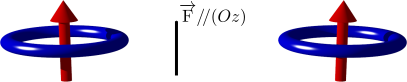
\includegraphics[width=.8\linewidth]{figures/double_torus.png}
\caption[Deux atomes circulaires côte à côte]{Représentation de deux atomes de Rydberg circulaires dont les orbites sont dans le même plan.
Les tores bleus représentent les orbites électroniques et les flèches rouges la direction du moment cinétique.
Si l'on imagine que le dessin est à l'échelle, alors les atomes sont ici séparés d'une distance d'environ \SIv{660}{\nm}.}
\label{fig:double_torus}
\end{figure}

Les règles de sélection étant toujours valides, le couplage se fait à l'ordre deux, et l'équation \eqref{eq:VdW_aacd} permet d'en extraire le coefficient de Van der Waals comme nous l'avons fait pour l'interaction 60S-60S.
%	Est-ce qu'on garde ça pour plus tard (circsim) ?\\
%	NOTA : ça correspond à la section 5.3 de Thanh, qui a l'air beaucoup plus fournie que ce que j'avais dans l'idée de mettre ici.\\
%		\noindent $C_6$ pour 50c-50c et $C_6/A_6$ avec les voisins \\
%		\noindent attention à l'anisotropie\\
		ICI, on ne traite le cas que de 50C-50C dans le plan de l'oribte. Le reste plus tard.
		Par contre, est-ce que ça a vraiment un sens comme calcul à champ nul ??

%--------------------------------------------------

%------------------------------------------------
%\chapter{Dispositif expérimental : une puce atomique pour des atomes de Rydberg}
%\label{chapter:setup}
%\chapter{Des atomes de Rydberg froids en environnement cryogénique}
\label{chapter:setup_coldatoms_Rydberg}

\section{Les atomes froids}
	\subsection{le cryostat et la puce}
	\subsection{séquence de piégeage et refroidissement}
		\noindent piégeage magnéto-optique
		\noindent piégeage magnétique
		\noindent refroidissement évaporatif jusqu'au BEC
	\subsection{imagerie atomique}
		\noindent optique d'imagerie
		\noindent imagerie par absorption
		\noindent tweaks : absorption no-log et réduction des franges
	\subsection{nuages typiques}
		\noindent quels MOTs, mélasses et nuages froids obtenus

\section{Excitation et détection d'atomes de Rydberg près d'une puce}
	\subsection{schéma d'excitation}
		\noindent laser et niveaux atomiques
	\subsection{schéma de détection}
		\noindent décrire la détection sélective en champ
	\subsection{problème de champs électriques et flash de Rb}
		\noindent vieilles raies larges et moches
		\noindent flash Rb
		\noindent belles raies fines
	\subsection{compensation et contrôle des champs}
		\noindent électrode Vcomp
		\noindent électrodes RF
	\subsection{manipulation et observation des Rydbergs}
		\noindent la spectroscopie microondes
%\chapter{Des atomes froids en environnement cryogénique}
%\label{chapter:setup_coldatoms}
%
%\section{Le cryostat}
%	\noindent description rapide du cryostat\\
%	\noindent feedthrough pour les courants de bobines et de puce ?
%
%\section{La puce et les bobines}
%	\noindent design de la puce et un petit mot sur la fabrication \\
%	\noindent bobines supras ?
%	
%\section{Séquence de piégeage et refroidissement}
%	\subsection*{Piégeage magnéto-optique}
%		\noindent 2d-mot, quad, u-mot, mélasse \\
%	\subsection*{Piégeage magnétique}
%		\noindent pompage optique et piège magnétique
%	\subsection*{Refroidissement évaporatif jusqu'au BEC}
%		\noindent dispositif de refroidissement RF
%
%\section{Imagerie atomique}
%	\subsection*{Optique d'imagerie}
%		\noindent front et side
%	\subsection*{L'imagerie par absoprtion}
%		\noindent traitement d'image : absorption et absorption "nolog" \\
%		\noindent mention de la réduction des franges ?
%	
%\section{Nuages typiques}
%	\noindent qu'obtient-t-on comme MOTs, mélasses, nuages ultra-froids avec notre dispositif
	
%		
%\section{excitation et détection d'atomes de Rydberg, contrôle du champ électrique}
%	\subsection*{schémas d'excitation}
%		Lhomond et CdF
%		
%	\subsection*{schémas de détection}
%		state selective ionization
%		signaux d'ionisation et toutes les subtilités
%		
%	\subsection*{contrôle du champ lors de l'excitation ET de la détection}
%		Lhomond et CdF
%		
%\section{problème des champs électriques près d'une puce}
%
%\section{spectroscopie microonde}

\chapter{Des atomes de Rydberg froids en environnement cryogénique}
\label{chapter:setup_coldatoms_Rydberg}

\section{Les atomes froids}
	\subsection{le cryostat et la puce}
	\noindent schéma et description du cryostat \\
	\noindent schéma et description de la puce supra et des bobines supra
	\subsection{séquence de piégeage et refroidissement}
		\noindent piégeage magnéto-optique : 2D-MOT, QUAD-MOT, U-MOT \\
		
		\noindent piégeage magnétique de Ioffe Pritchard : principe et potentiel créé par le fil Z (cf. code Mathematica Radia)\\
		
		\noindent refroidissement évaporatif jusqu'au BEC : principe de l'évaporation RF et fils d'évap sur la puce
		
	\subsection{imagerie atomique}
		\noindent optique d'imagerie : schéma optique et caractéristiques des caméras \\
		
		\noindent imagerie par absorption : transition sonde, intensité de saturation \\
		\noindent imagerie par réflexion sur la puce : spécificités de la géométrie et double absoprtion du faisceau sonde \\
		
		\noindent tweaks : absorption no-log et réduction des franges : qu'a-t-on utilisé comme méthodes de traitement pour améliorer notre imagerie $\rightarrow$ un paragraphe sur la réduction de franges et un(ou deux) paragraphe(s) sur l'absorption no-log et sa pertinence dans les mesures de mélasses.
		
	\subsection{nuages typiques}
		\noindent quels MOTs, mélasses et nuages froids obtenus : tailles, températures, nombres d'atomes, distance à la puce.

		
%\chapter{Dispositif expérimental : des atomes de Rydberg sur puce}
%\label{chapter:setup_ryd}
%
%\section{Excitation et détection d'atomes de Rydberg}
%	\subsection*{Schémas d'excitation}
%		\noindent schéma laser : schéma de niveaux (60s ou 50d) et schéma optique		
%	\subsection*{Schémas de détection}
%		\noindent state selective ionization
%		\noindent signaux d'ionisation et toutes les subtilités
%		
%\section{Problème des champs électriques près d'une puce}
%	\subsection*{L'élargissement Stark inhomogène}
%		\noindent raies de plusieurs dizaines de MHz de large, drift
%	\subsection*{Recouvrir la puce de rubidium}
%		\noindent dispositif dispensers et raies fines
%	\subsection*{Contrôle du champ électrique}
%		\noindent Lhomond et CdF, électronique de contrôle \\
%		\noindent électrodes RF pour la circularisation (Simion ?) 
%		
%\section{Spectroscopie microonde}
%	\noindent mention rapide des domaines de transition entre les niveaux de Rydberg
%	
\section{Excitation et détection d'atomes de Rydberg près d'une puce}

	\subsection{schéma d'excitation}
		\noindent schéma de niveau de l'excitation à deux photons (Raul.figIII.1) et caractéristiques de l'éexciation à deux photons (Rabi vs Detuning du niveau intermédiaire) \\
		\noindent schéma laser - puce - électrodes et petit mot sur la géométrie des faisceaux
		
		
	\subsection{schéma de détection}
		\noindent principe de la détection par ionisation \\
		\noindent implémentation : géométrie des électrodes d'ionisation, de déflexion et du channeltron \\
		\noindent avec une rampe de champ, on peut savoir quel niveau est détecté $\rightarrow$ principe des arrival times et note sur l'ionisation diabatique vs adiabatique. 
		
	\subsection{problème des champs électriques et flash de Rb}
	on travaille près d'une puce qui est une surface, et avec des objets ultra-sensibles -> ça peut créer des problèmes ! \\
		\noindent vieilles raies larges et moches : expliquer par l'effet Stark quadratique et l'élargiseement inhomogène. \\
		\noindent potentiel de contact et flash de Rb : dessins et schéma + dispensers et leur emplacement et boîte de protection \\
		\noindent c'est magiques, ça nous donne de belles raies fines !
		
	\subsection{compensation et contrôle des champs}
	c'est bien d'avoir' ces raies fines mais on veut contrôler le champ électrique le mieux possible
		\noindent électrode Vcomp et schéma de contrôle mixte excitation/détection. Le contrôle du champ sur $Oy$ c'est bien, ça permet de faire plein de trucs, mais il reste des gradients (au moins).\\
		
		\noindent si on veut faire encore mieux, il faut contrôler les champs selon $Ox$ et $Oy$ $\rightarrow$ électrodes RF :
		\\ schéma d'installation des électrodes
		\\ SIMION pour vérifier que ça permet de créer des champs y compris très près de la puce
		\\ en plus, ça servira de source de RF polarisée !!
		
	\subsection{manipulation et observation des Rydbergs}
\noindent C'est bien de détecter des Rydberg, mais il faut aussi pouvoir les manipuler et les caractériser.
Pour ça, on a un outil fabuleux : la spectroscopie microonde vers les niveaux voisins ! \\
schéma de niveaux ? schéma de dispositif ? \\
on peut mentionner ici qu'avec ça on a pu calibrer les champs électriques résiduels, et faire un qubit $60s-61s$ qui vit très longtemps.

\section*{Conclusion}
On a un dispositif lourd et complexe mais qui permet de faire beaucoup de belles choses avec des Rydbergs ultra-froids.

%-----------------------------------------------
%\chapter{Excitation optique d'atomes de Rydberg à bas $l$ et simulations}
%\label{chapter:60s}
\chapter{Interaction entre atomes de Rydberg sphériques et excitation de gaz dense}
\label{chapter:60s}
%Excitation optique d'atomes de Rydberg à bas $l$ et simulations
\noindent Les premières expériences que nous avons menées sur les interactions entre atomes de Rydberg ont eu lieu dans un nuage dense d'atomes froids au sein duquel sont excités de nombreux atomes vers l'état de Rydberg $\mathrm{60S}$.
Cela permet de mettre en évidence deux aspects différents de l'interaction au sein d'un nuage de Rydberg froid : l'influence des interactions sur la dynamique d'excitation des atomes de Rydberg et le mouvement des atomes en interaction au sein du nuage.

Après un rappel de la forme de l'interaction dipolaire, nous en expliquerons les effets sur le mouvement des atomes de Rydberg dans le nuage et sur la dynamique d'excitation de ces mêmes atomes.
Nous présenterons ensuite une expérience de spectroscopie optique mettant en evidence ces effets.

Le modèle numérique de simulation que nous avons développé nous permettra de confirmer notre compréhension de ces effets et leur importance.
Enfin, nous présenterons une expérience de spectroscopie microonde permettant de sonder plus précisément les énergies d'interactions dans un nuage d'atomes de Rydberg, à différents moments de son expansion.

%\section{Régimes d'excitation en nuage dense : blocage et facilitation}
\section{Les effets de l'interaction dipolaire en nuage dense}


	\subsection{Rappels sur l'interaction dipolaire}
\noindent L'interaction dipolaire entre deux atomes de Rydberg dans le même état $\ket{a}$ et séparés d'une distance $r$ prend la forme suivante, établie en \ref{subsec:interaction_same_level} :
\begin{equation}
\label{eq:Vdd_aa}
\hat{V}_{dd}(r) = \frac{hC_6}{r^6} \cdot \ket{aa}\bra{aa}.
\end{equation}
Ce potentiel d'interaction agit donc comme un simple déplacement de l'énergie de la paire d'atomes par une quantité $E_{int} (r)=hC_6/r^6$ .
Nous travaillerons dans l'hypothèse que cette interaction de Van der Waals est additive pour un ensemble de $N$ atomes.
Ainsi, l'atome $i$ subira la somme des interactions de paire avec les autres atomes $j$ de l'ensemble :
\begin{equation}
\label{eq:Eint_isum}
E_{int}(i) = \sum_{j\neq i} E_{int}(i,j) = \sum_{j\neq i} E_{int}(r_{ij}) = h C_6 \cdot \sum_{j \neq i} \frac{1}{r_{ij}^6}.
\end{equation}
Cette hypothèse d'additivité est valide dès lors que l'on se limite au second ordre du couplage dipôle-dipôle \cite{ENS_CHIPINTERACTION15,MX_TELLER_ADDITIVEVDW}.
La figure \eqref{fig:VdW_sum_N} représente un tel ensemble d'atomes en interaction.
%
\begin{figure}[h]
\centering
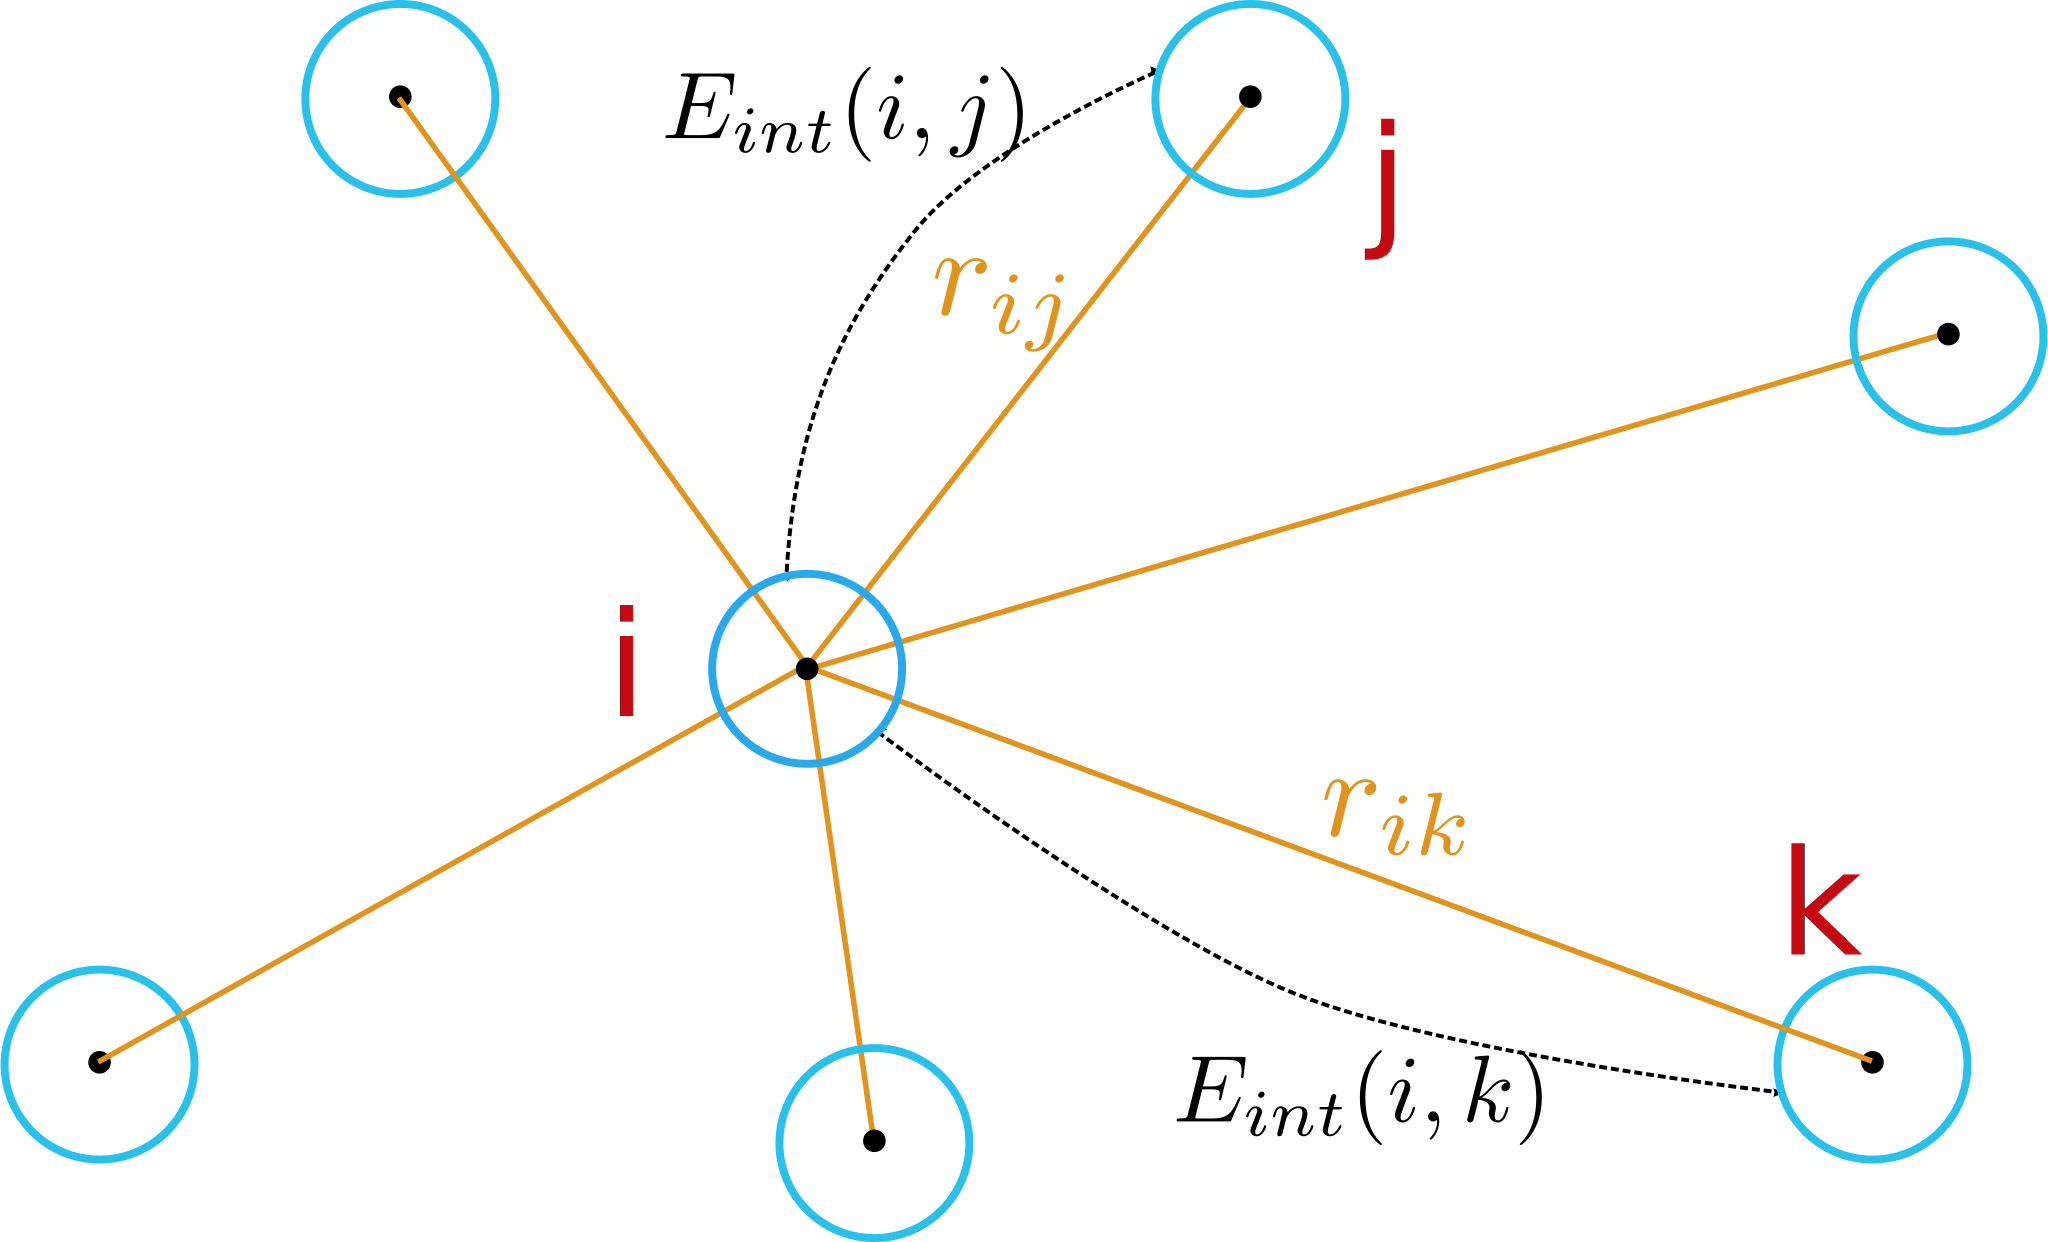
\includegraphics[width=0.6\linewidth]{figures/low_l/Natomes}
\caption[Ensemble de $N$ atomes de Rydberg en interaction Van der Waals]
{Ensemble de $N$ atomes de Rydberg en interaction Van der Waals.
L'énergie d'interaction de chaque atome est la somme de ses énergies d'interaction de paire avec tous les autres.
}
\label{fig:VdW_sum_N}
\end{figure}

	\subsection{Mouvement des atomes au sein d'un gaz dense de Rydberg}
	\noindent Le premier effet des interactions dipolaires au sein d'un nuage d'atomes de Rydberg est un effet mécanique.
Comme nous l'avons vu en \ref{sec:interacting_rydbergs}, l'interaction est répulsive entre atomes de Rydberg dans le même niveau $\ket{\mathrm{nS}}$.
Ainsi, deux atomes de Rydberg en interaction dipolaire subiront chacun une force répulsive, directement dérivée de leur énergie d'interaction,
\begin{equation}
\label{eq:repuls_2atoms}
F = - \frac{d E_{int}}{dr}  = + \frac{6hC_6}{r^7}.
\end{equation}
Cela équivaut à un traitement classique de l'effet mécanique de l'interaction dipolaire, bien que le calcul de cette même interaction ne le soit pas.
Cela nous est permis par la forme simple de l'interaction dipolaire entre deux atomes dans le même état de Rydberg, donnée par l'équation \eqref{eq:Vdd_aa}, qui consiste en un simple déplacement d'énergie du niveau de paire $\ket{aa}$.

Prenons l'exemple de deux atomes dans le niveau $\mathrm{60S}$, séparés d'une distance de $\SI{5}{\um}$ : leur énergie d'interaction vaut $hC_6/r^6 = h\cdot {\SI{137.6}{\GHz\raiseto{6}\um}}/(\SI{5}{\um})^6 = \SI{8.8}{\MHz}$.
Ils se repoussent donc avec une force valant %$6hC_6/r^7 = 6h\cdot \SI{137.6}{\GHz\raiseto{6}\um}/(\SI{5}{\um})^7 = \SI{6.97e-27}{\mega\newton} = \SI{6.97e-21}{\newton}$.
$6hC_6/r^7 =\SI{6.97e-21}{\newton}$.
Étant donnée la masse du rubidium, cette force répulsive correspond à une accélération valant $F/m_{Rb87} = \SI{4.83e4}{\m\per\s\squared}$, soit $\num{5000}$ fois plus que l'accélération de la gravité.
Une intégration numérique grossière permet d'extraire un ordre de grandeur du déplacement des atomes : en $\SI{20}{\us}$, ils auront presque atteint leur vitesse relative maximale de $\SI{0.284}{\m\per\s}$ et en $\SI{10}{\us}$ seulement la distance qui les sépare aura augmenté de $\SI{1.75}{\um}$.
Leur énergie d'interaction aura par là chuté d'un facteur $\SI{5.77}{}$, ce qui constitue une modification considérable du système.

La généralisation à $N$ atomes se fait en additionnant vectoriellement les forces répulsives dues à chaque interaction de paire :
\begin{equation}
\label{eq:repuls_Natomes}
\vec{F}(i) =  \sum_{j\neq i} -\vec{\nabla}E_{int}(i,j)
= \sum_{j\neq i} \frac{6hC_6}{r_{ij}^7} \cdot \frac{-\vec{r}_{ij}}{r_{ij}}
= - 6hC_6 \cdot \sum_{j\neq i} \frac{\vec{r}_{ij}}{r_{ij}^8}.
\end{equation}
%
Cette force répulsive décroît très vite avec la distance.
On s'attend ainsi à ce que deux atomes de Rydberg en interaction s'accélère mutuellement pendant un temps court, se propageant ensuite balistiquement dans des directions opposées.
C'est ce que confirme l'exemple de la paire $\ket{\mathrm{60S,60S}}$ précédemment cité.
Il est intéressant de noter qu'au sein d'un nuage d'atomes de Rydberg, les atomes du c\oe ur  sont repoussés par les interactions dipolaires de tous les côtés.
Les atomes du bord du nuage seront alors expulsés en premier, puis petit à petit les atomes plus au centre pourront commencer à se déplacer.
Le nuage subit ainsi une expansion hydrodynamique non triviale, que nous mesurerons expérimentalement et simulerons numériquement.

	\subsection{Deux régimes d'excitation en interaction dipolaire forte}\label{subsec:excitation_bloc_facil}
	%Le blocage dipolaire et la facilitation}

\noindent Les interactions dipolaires ont également une influence importante sur l'excitation d'un ensemble dense d'atomes de Rydberg.	
En effet, la présence d'un atome de Rydberg conditionne l'excitation ultérieure d'autres atomes de Rydberg dans son voisinage.
Lorsque l'excitation est faite à résonance, cet effet est connu sous le nom de \og blocage dipolaire \fg{}.

	\subsubsection*{Blocage dipolaire et super-atomes}
\noindent Le mécanisme du blocage dipolaire est illustré en figure (\ref{fig:dip_block} a)).
Considérons deux atomes dans l'état fondamental $\ket{g}$, séparés d'une distance $r$.
L'état de la paire est alors $\ket{g,g}$.
Un laser est accordé à résonance pour exciter l'un quelconque de ces deux atomes vers le niveau de Rydberg $\ket{ry}$.
L'état de la paire devient ainsi $\ket{g,ry}$.% ou $\ket{ry,g}$.
Si l'on souhaite exciter le second atome vers le niveau $\ket{ry}$, alors il faut considérer l'énergie nécessaire à la transition $\ket{g,ry} \rightarrow \ket{ry,ry}$.
Or ce dernier état de paire subit un déplacement d'énergie dû à l'interaction de Van der Waals
%
\begin{equation}
\label{eq:DeltaE_block}
\Delta E_{\ket{ry,ry}}(r) = E_{\ket{ry,ry}}(r)-E_{\ket{ry,ry}}(\infty)
= E_{int}(r).
\end{equation}
%
Le laser, qui était à résonance avec la transition $\ket{g,g}\rightarrow\ket{g,ry}$, n'est ainsi plus à résonance avec la transition $\ket{g,ry}\rightarrow\ket{ry,ry}$.
L'excitation du second atome vers un niveau de Rydberg s'en trouve bloquée.

\begin{figure}[!h]
\centering
\includegraphics[height=.3\textheight]{figures/low_l/dip_block}
\caption[Mécanisme du blocage dipolaire]{
Illustration du mécanisme de blocage dipolaire.
\textbf{a)} Diagramme d'énergie des niveaux de paire à zéro, un ou deux atomes excités, en fonction de la distance interatomique $r$.
$\ket{g}$ est le niveau fondamental et $\ket{ry}$ le niveau de Rydberg considéré.
Aux courtes distances, l'interaction dipolaire déplace l'excitation du deuxième atome vers le niveau de Rydberg hors de résonance avec le laser ayant excité le premier atome.
$\gamma$ représente la largeur spectrale de la raie d'excitation à un atome, $E_{int}$ l'énergie d'interaction entre deux atomes de Rydberg et $r_b$ le \og rayon de blocage \fg{}.
\textbf{b)} Généralisation à un ensemble d'atomes. Les points bleus sont des atomes dans l'état fondamental et les points rouges sont des atomes de Rydberg.
Le mécanisme de blocage empêche l'excitation de deux atomes de Rydberg dans un même sphère de rayon $r_b$, représentée par les disques rouges.
}
\label{fig:dip_block}
\end{figure}

Le laser d'excitation n'est pas infiniment fin spectralement et l'effet de blocage dipolaire sera limité par sa largeur spectrale.
On peut en effet considérer que le laser est résonant avec la transition dès lors que le désaccord entre eux est inférieur à la demi-largeur spectrale $\gamma/2$ de la raie d'excitation.
Nous définirons ainsi le \og rayon de blocage \fg{} $r_b$ comme étant la distance en-deçà de laquelle le désaccord est supérieur à la demi-largeur spectrale :
\begin{equation}
\label{eq:def_rayon_bloc}
\Delta E_{int}(r_b) = \gamma /2 
\end{equation}
%
Dans le cas qui nous intéresse, l'interaction dipolaire a une forme de Van der Waals en $1/^6$, permettant de réécrire l'équation \eqref{eq:def_rayon_bloc} sous la forme
\begin{equation}
\label{eq:def_rayon_bloc}
\frac{C_6}{r^6} = \gamma /2 \text{ , soit } r_b = \sqrt[6]{\frac{C_6}{\gamma /2}}
\end{equation}
%
Le mécanisme de blocage est donc effectif à l'intérieur d'un \og volume de blocage\fg{} autour de chaque atome de Rydberg déjà excité.
Ce volume de blocage est une sphère de rayon $r_b$, représentée en figure (\ref{fig:dip_block} b)).

Revenons au cas de deux atomes :
il existe deux états de paire à une excitation, qui sont $\ket{g,ry}$ et $\ket{ry,g}$.
Ces deux états sont dégénérés et le laser couple le niveau fondamental $\ket{g,g}$ indifféremment à $\ket{g,ry}$ et à $\ket{ry,g}$, avec même une fréquence de Rabi $\Omega$.
La combinaison symétrique $\ket{D} = \left( \ket{g,ry} + \ket{ry,g} \right) / \sqrt{2}$, appelée état collectif de Dicke des deux atomes, est alors couplée à l'état fondamental avec une fréquence de Rabi augmentée $\Omega\sqrt{2}$.
Ce facteur d'accroissement a été mis en évidence expérimentalement par le groupe de A. Browaeys et P. Grangier \cite{MX_BROWAEYS_COLLECRABIBLOCK}, en observant deux atomes piégés dans des pinces optiques.

L'idée se généralise au cas à $N$ atomes en utilisant encore une fois le modèle de Dicke.
Dans un rayon de blocage contenant $N_b$ atomes, l'état du système oscille entre l'état fondamental et l'état de Dicke à une excitation, toute excitation supplémentaire étant interdite par blocage dipolaire.
Cette oscillation se fait cette fois avec une fréquence de Rabi $\Omega\sqrt{N_b}$.
Un modèle simple de ce phénomène consiste à voir l'ensemble de ces $N_b$ atomes comme un unique \og super-atome \fg{} ayant un moment de transition dipolaire $\sqrt{N_b}$ plus grand  que celui d'un atome isolé.
Ce modèle de super-atome a été exploité avec succès pour expliquer des observations expérimentales par les groupes d'I. Bloch \cite{MX_BLOCH_SUPERATOM} et de H. Ott \cite{MX_OTT_SUPERATOM}.


	\subsubsection*{Excitation facilitée et agrégats de Rydberg}
	
\begin{figure}[!h]
\centering
\includegraphics[height=.3\textheight]{figures/low_l/dip_facil}
\caption[Mécanisme de facilitation]{
Mécanisme de facilitation
}
\end{figure}

		\noindent les deux régimes d'excitation déterminée par les interactions :\\
		explication du blocage dipolaire, et des effets qui le limitent (ailes de la gaussienne du nuage) \\
		pourquoi c'est difficile dans un BEC : mention du Pfau shift \\
		mention de la négligeabilité des excitations de paires ?

\section{Spectroscopie optique du nuage}
	\subsection{Description de la manip}
		\noindent spectres à différents temps d'interaction\\
		ou $N_rydberg$ en fonction du temps d'interaction pour différents detunings
		
	\subsection{Données : élargissement de la raie laser par interactions}
		\noindent conséquence de la facilitation
		
\section{Modèle de la dynamique d'excitation}
	\subsection{Simulations}
		\noindent modèle d'équation de taux\\
		\noindent résultats de simulations comparés aux manips\\
	\subsection{Les limites du modèle}
		%\noindent question du chauffage
		\noindent photons thermiques et apparition de niveaux $p$ \\
		LIRE T. PORTO
		
\section{Spectroscopie microonde du nuage : voir le mouvement}
	\subsection{Description de la manip}
		\noindent spectroscopie 60s-57s et son spectre d'excitation : comment cela nous donne accès au spectre des énergies d'interaction\\
		sonder le nuage à différents moments de son explosion
	\subsection{Données et accord avec les simulations}
		\noindent présenter les courbes de Raul.IV.3.2
		

\section*{Conclusion}
		\noindent il faut prendre en compte le mouvement, mais aussi les transferts thermiques vers les niveaux $p$
		
%\section{Spectroscopie microonde du nuage}
%	\subsection*{Spectre des énergies d'interaction du nuage}
%		\noindent détails sur la spectro 60s-57s, dont la quasi absence de terme d'échange dans l'interaction
%	\subsection*{Mouvement du nuage de Rydbergs}
%		\noindent Le gaz gelé ne marche pas !

%\chapter{Les atomes de Rydberg circulaires en interaction : vers un simulateur quantique}
%\label{chapter:circsim}
\chapter{Les atomes de Rydberg circulaires en interaction : vers un simulateur quantique}
\label{chapter:circsim}

Intro : pourquoi envisager les Rydberg circulaires comme plateforme de simulation ?

\section{Les interactions dipôle-dipôle entre atomes de Rydberg circulaires}

\section{Le hamiltonien $XXZ$ simulé}
	\subsection{Mise sous forme XXZ}
	\subsection{"Tunabilité" des interactions}
		Comment justifier le domaine de champs électrique et magnétique statiques dans lequel on se place, avant d'avoir parlé du problème de la durée de vie ??
	\subsection{Quelle physique ? Diagramme de phase}

\section{Principes techniques du simulateur}
	\subsection{Piégeage laser des Rydberg circulaires}
	\subsection{Préservation des états de Rydberg}
		\subsubsection*{Temps de vie dans l'espace libre}
		\subsubsection*{Inhibition de l'émission spontanée}
		\subsubsection*{Problème du mixing et solution}
	\subsection{Préparation déterministe d'une chaîne}

\newpage
Reprendre le PRX

%\chapter{Excitation d'atomes de Rydberg circulaires et piégeage laser}
%\label{chapter:50c}
\chapter{Des atomes de Rydberg circulaires sur puce}
\label{chapter:50c}
%Excitation d'atomes de Rydberg circulaires et piégeage laser

\section{Comment exciter des atomes de Rydberg circulaires}
	\subsection*{Les niveaux atomiques du fondamental au Rydberg circulaire}
		\noindent schéma de niveaux et Stark maps
	\subsection*{Spectroscopie 5s-50d}
		\noindent en champ nul et en champ non-nul -> choix de $m_j$
	\subsection*{Spectroscopie 50d-50f}
		\noindent en champ nul et en champ non-nul -> choix de $m_l$ et problème d'élargissement
	\subsection*{Le passage adiabatique}
		\noindent et le dispositif radio-fréquence

\section{Comment caractériser les atomes de Rydberg circulaires}
	\subsection*{Spectroscopie microonde}
		\noindent 50c-51c et optimisation de la RF\\
		\noindent 50c-49c ?
	\subsection*{Temps de vie}
		\noindent temps de vie théorique, temps de vie mesuré, température effective
	\subsection*{Temps de cohérence}
		\noindent franges de Ramsey
	

%\section{Théorie de la force pondéro-motrice appliquée aux 50C} -> goes to chapter:circsim
%	\noindent et description du laser de piégeage

\section{Éjectable : Première évidence du piégeage des atomes circulaires}
	\noindent chute par gravité et/ou expansion du nuage compensée par un tube de lumière


\chapter*{Conclusion}\label{chapter:concl}
\addcontentsline{toc}{chapter}{Conclusion}
\markboth{Conclusion}{Conclusion}
\include{}%0_intro}

%\phantomsection
%\titleformat{\part}[block]
%{\bfseries\fontsize{26}{28}\selectfont}
%{}
%{10pt}
%{
%	\begin{tikzpicture}[remember picture, overlay]
%	\node[anchor=south west, inner sep =0pt, outer sep =25pt](partnum) at (0,3){\partnumfont\itshape };
%	\end{tikzpicture}\parbox[c]{.95\textwidth}%\justify
%}
\part*{Annexes}
\appendix
\renewcommand{\chaptermark}[1]{\markboth{\appendixname\ \thechapter: #1}{}}

\renewcommand{\bibname}{References}
\printbibliography

\include{}%6_appendix}
\backmatter
\include{}%0_intro_fr}
\end{document}